\documentclass[]{report}

\usepackage{amsmath}
\usepackage{graphicx}
\usepackage{algorithm}
\usepackage{hyperref}       % hyperlinks
\usepackage{url}            % simple URL typesetting
\usepackage{booktabs}       % professional-quality tables
\usepackage{amsfonts}       % blackboard math symbols
\usepackage{nicefrac}       % compact symbols for 1/2, etc.
\usepackage{microtype}      % microtypography
\usepackage{amssymb}
\usepackage{amsmath}
\usepackage[utf8]{inputenc}
\usepackage[english]{babel}
%\usepackage{subfigure}
%%\usepackage{tikz}
%\usepackage{algorithm}
\usepackage{algpseudocode}
%\usepackage{graphicx}
%\usepackage{subfig}
\newcommand{\tif}{\textit}
\newcommand{\tbf}{\textbf}
% Title Page
\title{Hamiltonian Monte Carlo}
\author{Bradley Gram-Hansen}


\begin{document}
\maketitle


\section{Intro to HMC MCMC}

Following Neal 2011 Chapter 5 Handbook of MCMCM
\subsection{Metropolis-hastings algorithm}
The Metropolis hastings algorithm is the work horse of Monte Carlo Markov Chain (MCMC) methods, It relies on a simple reject and accept criteria for determining whether or not we should proceed to some next state. If our state is accepted, but does not satisfy the full criteria then a probability is associated with that state, and if that probability exceeds the one sampled from a given cut off, usually determined by sampling from a uniform distribution then it is accepted, else rejected. 

\begin{algorithm}
\caption{Metropolis-Hasting algorithm}
\begin{algorithmic}[1]
	\State  $x^{0} \sim P_{0}(x)$ \Comment{Where $p(x)$ is the proposed initial distribution}
		\For {$s = 0,1,2,\ldots$}
		\State $ x \gets x^{s} $
		\State $ x^{'} \sim Q(x^{'}|x)$
		\State $a = \frac{\tilde{P}(x')Q(x|x')}{\tilde{P}(x)Q(x'|x)}$ \Comment{Acceptance ratio}
		\State $r = min(1, a) $ \Comment{Acceptance condition}
		\State $u \sim  U(0,1)$ 
		\State $x^{s+1} = \begin{cases}
		x' \text{ if $u < r$}\\
		x^{s} \text{ if $u \geq r$}
		\end{cases}$
		\EndFor
\end{algorithmic} 
\end{algorithm}

\subsection{HMC for MCMC}

In a top level view Hamilton Monte Carlo for Monte Carlo Markov Chain (HMC MCMC) is a two step process. In step one we define a Hamiltonian function in terms of the probability distribution from which we wish to sample from. We introduce a position variable, $q$ and momentum variable $p$, where $p$ is an auxiliary variable that typically has a Gaussian distribution.  All $p$'s are assumed independent. 
In step two, the HMC alternates simple updates for the momentum variables with Metropolis updates. This enables us to propose a new state by computing a trajectory according to Hamiltonian dynamics, implemented with the leapfrog method. 
\subsubsection{Prerequisites}
The Hamiltonian of a physical system is defined completely with respect to the position $q$ and $p$ momentum variables, which span the phase space of the system. The Hamiltonian is the Legendre transform of the Lagrangian and gives us the total energy in the system. It is defined as follows: 
\begin{equation}
\label{eq:hamiltonian}
 H(\textbf{q},\textbf{p}) = \sum_{i = 1}^{d}\dot{q}_{l}p_{l} - L(\textbf{q}, \textbf{\.{q}}(\textbf{q}, \textbf{p}))
\end{equation}
where $d$ is the system dimensions, and so the full state space with has $2d$ dimensions.  
Thus, for simplicity, if we set $d = 1$ we can derive the Hamiltonian equations as follows:\begin{equation}
\frac{\partial H}{\partial p} = \dot{q} + p\frac{\partial \dot{q}}{\partial p} - \frac{\partial L}{\partial \dot{q}}\frac{\partial \dot{q}}{\partial p} = \dot{q} \end{equation}
and 
\begin{equation}
\frac{\partial H}{\partial q} = p\frac{\partial \dot{q}}{\partial q} - \frac{\partial L}{\partial q} - \frac{\partial L}{\partial \dot{q}}\frac{\partial \dot{q}}{\partial q} = - \frac{\partial L}{\partial q}= -\dot{p}  \end{equation}
and the process is the same for more than one dimension. 
We can write \ref{eq:hamiltonian}\ more succinctly as:
\begin{equation}
\label{eq:hamreduced}
H(\textbf{q}, \textbf{p})  = K(p) + U(q)
\end{equation}
where $K(p)$ represents our kinetic energy and $U(q)$ is the potential energy.

Within the HMC MCMC framework the ''positions", $q$, are the variables of interest and for each position variable we have to create a fictitious ''momentum", $p$. For compactness let $z = (q,p)$. The potential energy $U(q)$ will be the minus of the log of the probabilty density for the distribution of the position variables we wish to sample, plus \textbf{any} constant that is convenient.  The kinetic energy will represents the dynamics of our variables, for which a popular form of $K(p) = \frac{p^{T} M^{-1} p}{2}$, where $M$ is symmetric, positive definite and typically diagonal. This form of $K(p)$ corresponds to a minus the log probability of the zero mean Gaussian distribution with covariance matrix $M$. For this choice we can write the Hamiltonian equations, for any dimension $d$, as follows:
\begin{align}
\dot{q}_{i} &= \frac{dq_{i}}{dt} = [M^{-1}p]_{i} \\
\dot{p}_{i} &= \frac{dp_{i}}{dt} = -\frac{\partial U}{\partial q_{i}}
\end{align}

To view the Hamiltonian in terms of probabilities, we use the concept of the canonical distribution from Statistical mechanics to construct our pdf. Thus, the distribution that we wish to sample from can be related to the potential energy via the canonical distribution as:
\begin{equation}
\label{eq:canonical}
P(z) = \frac{1}{Z}\exp\left(\frac{-E(z)}{T}\right)
\end{equation}
As the Hamiltonian is just an energy function we may can insert \ref{eq:hamreduced}\ into our canonical distribution \ref{eq:canonical}\, which gives us the joint density:
\begin{equation}
P(q,p) = \frac{1}{Z}\exp(-U(q))\exp(-K(p)  
\end{equation}
where $T = 1$ is fixed. And so we can now very easily get to our target distribution $p(q)$, which is dependent on our choice of potential $U(q)$, as this expression factorizes in to two independent probability distributions. 
We characterise the posterior distribution for the model parameters using the potential energy function: \begin{equation}
U(q) = -\log[\pi(q)L(q|D)]
\end{equation}
where $\pi(q)$ is the prior distribution, and $L(q|D)$ is the likelihood, not the Lagrangian, of the given data $D$. 

\subsection{The Algorithm}

\subsubsection{The leapfrog method}
The leapfrog method enables reduced error and allows us to dicretize Hamiltons equations, so that we can implement them numerically. 
We start with a state at $t = 0$ and then evaluate at a subsequent time $t + \epsilon , \hdots, t + n\epsilon$, where $\epsilon$ is the step in which we increase and $n$ is the number of time steps. 

\begin{align}
p_{i}(t + \frac{\epsilon}{2}) &= p_{i}(t) - \left(\frac{\epsilon}{2}\right)\frac{\partial U(q(t))}{\partial q_{i}} \\
q_{i}(t + \epsilon) &= q_{i}(t) + \epsilon\frac{\partial K(p(t + \frac{\epsilon}{2}))}{dp_{i}}\\
p_{i}(t + \epsilon) &= p_{i}(t + \frac{\epsilon}{2}) - \left(\frac{\epsilon}{2}\right)\frac{\partial U}{\partial q_{i}}\\
\end{align}
\footnote{For the usual choice of kinetic energy, we have $\frac{\partial K(p + \frac{\epsilon}{2})}{dp_{i}} = \frac{p_{i}(t + \frac{\epsilon}{2})}{m_{i}}$}

For the leapfrog method the local error, error after one step, is of $\mathcal{O}(\epsilon^{2})$ and a global error, error after simulating for some fixed time interval s, which requires $\frac{s}{\epsilon}$ is $\mathcal{O}(\epsilon^{3})$
\subsubsection{Some initial points of notice}
Neals implementation of the HMC can only be used to sample from continuous distributions on $\mathbb{R}^{d}$ for which a density function can be evaluated.\\
We must be able to compute the partial derivative of the log of the density function. The derivaties must exists at the points at which they are evaluated [\textbf{Automatic differention}]

HMC samples from the canonical distribution for $q$ and $p$. $q$ has the distribution of interest as specified by the potential $U(q)$. 
The distribution of the $p$'s can be chosen by us and are independent of the $q$'s. 
The $p$ components are specified to be independent, with component $p_{i}$ having variance $m_{i}$.
The kinetic energy $K(p) = \sum_{i =1}^{d}\frac{p_{i}^{2}}{2m_{i}}(q(t + \epsilon))
$

\subsubsection{The steps}

\begin{enumerate}
	\item Step 1: Changes only the momentum
	\item Step 2: May change both position and momentum
\end{enumerate}
Both steps leave the canonical distribution of (q,p) invariant, hence the distribution remains invariant.

In \textbf{Step 1} we first draw the $p_{i}$ randomly from their Gaussian distribution independently of the current values of the position values. 
In \textbf{Step 2} a Metropolis update is performed, using the Hamiltonian dynamics to propose a new state. Starting with the current state $(q,p)$, Hamiltonian dynamics is simulated for $L$ steps using the leapfrog method, with a stepsize of $\epsilon$. $L$ and $\epsilon$ are parameters of the mnodel that need to be tuned.\\
The momentum vairables at the end of this $L$-step trajectory are then negated, giving s proposed state $(q^{*}. p^{*})$. This proposed state is accepted as the next state in the Markov Chain with probability: \begin{equation}
\min[1, \exp(-H(q^{*}, p^{*}) + H(p,q)] = \min[1, \exp(-U(q^{*}) + U(q) - K(p^{*}) + K(p))]
\end{equation} 
If the proposed state is rejected, then the next state is the same as the current state and is counted again when calculating the expected value of some function. 
The negation of the momentum variables at the end of the trajectory makes the Metropolis proposal symmetrical, as needed for the acceptance probability above to be valid. This negation need not be done in practice, since $K(p) = K(-p)$, and the momentum will be replaced before it is used again, in the first step of the next iteration.\label{key}

\begin{algorithm}
	\label{alg:simpHMC}
	\caption{Simple Hamiltonian Monte Carlo MCMC}
	\begin{algorithmic}[1]
	\Procedure{HMC single iteration}{$\epsilon$, $L$, $q_{current}$}
		\State $ q \gets q_{current}$
		\State $ p \sim \mathcal{N}(len(q),0,1)$
		\State $ p_{current} \gets p$
		\State $ p \gets p - \frac{\epsilon}{2}\nabla_{q} U(q)$ \Comment{make half step for momentum} 
		\For{$i \text{ in } 1:L$}
		\State $q \gets q + epsilon * \nabla_{p} K (p(t + \frac{\epsilon}{2}))$ \Comment{make full step for the position} 
		\If{$i != L$}
		\State $p \gets p- \epsilon \nabla_{q} U(q)$
		\EndIf
		\EndFor
		\State $p - \frac{\epsilon}{2}\nabla_{q} U(q)$ \Comment{Half step for momentum}
		\State $p \gets - p$ \Comment{Ensuring symmetry of Metropolis proposal}
		\State $U_{current} \gets U(q_{current})$
		\State $U_{proposed} \gets U(q)$
		\State $K_{current} \gets \frac{1}{2} p_{current} \cdot p_{current} $
		\State $K_{proposed} \gets \frac{1}{2} p \cdot p$
		\State $ u \sim Uniform(0,1)$
		\If{$u < exp(U_{current} - U_{proposed} + K_{current} - K_{proposed})$}
		\State $\text{return } q \gets q$ \Comment{Accept}
		\Else
		\State $\text{return } q_{current} \gets q_{current}$ \Comment{Reject}
		\EndIf
	\end{algorithmic} 
\end{algorithm}
A function that implements a single iteration of the HMC algorithm is given in algorithm 2. There are three additional functions within this iteration: $U$, which returns the potential energy given a value for $q$,  $\nabla U$, which returns the vector of partial derivatives of $U$ given $q$ and $\nabla K$, which returns the vector of partial derivatives of $K$ given $p$. Other arguments are the stepsize, $\epsilon$, for leapfrog steps, the number of leapfrog steps in the trajectory, $L$, and the current position, $q_{current}$, that the trajectory starts from. Momentum variables are sampled within this function, and discarded at the end, with only the next position being returned. 

\subsection{Tuning the HMC}

We need to select suitable parameters $\epsilon$ and $L$, which together determine the length of the trajectory in fictitious time $\epsilon L$  

\section{Automatic differentiation AD}
Automatic differentiation is quite different from both Numerical and Analytical differentiation. It is, in a very loose sense a hybrid of the two, that is optimal for computational performance. It works by systematically applying the chain rule of differential calculus at the elementary operator level, enabling us to generate numerical derivative evaluations through the accumulation of values.   
This “interleaving” idea forms the basis of AD and provides an account of
its simplest form: apply symbolic differentiation at the elementary operation
level and keep intermediate numerical results, in lockstep with the evaluation
of the main function. This is AD in the forward accumulation mode

\subsection{Automatic Differentiation in Pytorch}
To use autodiff in pytorch we make use of the \textit{autograd} package. it provides automatic differentiation for all operations on tensors. It is a \textbf{define-by-run framework}, which means brackprop is defined by how your code is run and that every single iteration \textbf{can be} different. 

\subsubsection{Variable}

\textit{autograd.Variable} is the central class of the package. Once you finish your call \textit{.backward()} and have all the gradients computed automatically. You can access the raw tensor through the \textit{.data} attribute, while the gradient w.r.t to that variable is accumulated in \textit{.grad}. 
Another important class is \textit{autograd.Function}, which is interconnected with \textit{Variable}. Together they build an \textbf{acyclic} that encodes the complete history of the computation. Each variable has a \textit{.creator} attribute that references a \textit{Function} that has created the \textit{Variable}.  
\begin{figure}[!]
\centering
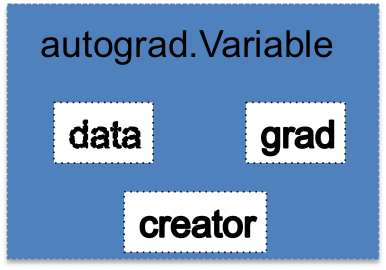
\includegraphics{../Pytorch_learning/autograd}\caption{Variable}
\end{figure}

\subsubsection{Gradients}

To calculate \textbf{gradients} from our \textit{Variable} object we apply the method \textit{<newVariable>.backward()} (where \textit{newVariable} is created from the original variable) and then extract the attribute \textit{<Variable>.grad} from the original variable. We are interested in the relation between the \textit{newVariable} and the \textit{Variable} as composition of functions, and the gradients of those functions evaluated at the a particular point. 


\subsection{Neural Networks in Torch}

Using the \textit{torch.nn} package, we can develop a NN. The \textit{torch.nn} package is dependent upon the \textit{autograd} package, to define models and differentiate them.  The \tif{nn.Module} contains layers and a method \tif{.forward(input)} returns the \tif{.output}. 

\subsubsection{Training Procedure}
\begin{enumerate}
	\item Define the NN that has some learnable parameters (or weights) 
	\item Iterate over a dataset of inputs
	\item Process input through the network
	\item Compute the loss ( how far is the output from being corrected)
	\item Propagate gradients back into the network's parameters
	\item Update the weights of the network, using a update rule
\end{enumerate} 

A simple update rule might be of the form: $weight = weight - learningRate \times gradient$. When using PyTorch, you always have to define the \tif{forward} function, but once that is done, PyTorch, using \tif{autograd}, will automatically define the \tif{backward} function.  The learnable parameters of the model can be recalled by using \textit{<class\_name\_for\_nn>.parameters()}. See \tbf{blitztor.py} for more details.\\

\tbf{Important note: } \tif{torch.nn} only supports mini-batches, the entire \tif{torch.nn} package only supports inputs that are a mini-batch of samples and not a single sample.\\

To load data in to pytorch, we load data in via an nparray and convert this array into a \textit{torch.*Tensor}.
For loading audio, use scipy and librosa. For loading text either raw Python an Cython based loading, ir NLTK and SpaCy. For vision Pytorch has the \tif{torchvision} package.  
  
 
\subsubsection{Loss function}

The loss function takes the (output, target) pairs of inputs, and computers a value that estimates how far away the output is from the target, under some measure. The Pytorch library contains many different loss functions, see documentation. See \tbf{blitzor.py} for more details.
To give all \tif{Variables} there specified gradients, up to their node in the tree, 
we simply call \tif{loss.backward()} and that accumulates all \tif{.grad}'s to calculate the gradient for the different variables, w.r.t the loss.
This also enables us to backprop the error through the network, although the existing gradients will need to be cleared. Else, you will be double adding. To zero we use the command \textit{<neural\_net\_object>.zero\_grad()}.

\subsubsection{Backprop}
To get any Variables derivative w.r.t the loss, we call, after doing \tif{loss.backward()}, \tif{<network\_name>.<Variable\_name>.\{other\_properties\}.grad}

\subsubsection{Updating the Weights}
Using the \textit{torch.optim} package we can use an array of optimizers, including SGD. See documentation. 


\end{document} 
